%************************************************
\chapter{Experimental Setup}
\label{ch:detector}
%************************************************

\section{Introduction}
\label{sec:detector_introduction}

Our experimental data was collected from the ATLAS particle detector in the Large Hadron Collider (LHC).
The following section will introduce LHC and the ATLAS particle detector.

\section{The Large Hadron Collider}
\label{sec:detector_LHC}

The Large Hadron Collider (LHC) was built in the border between France and Switzerland by the European Organization for Nuclear Research (CERN).
It is a circular particle collider under the ground with circumference 27 km.
Two beams of protons will be accelerated in opposite directions, and then these two beams will collide with each other at the collision point. The center-of-mass energy of the two beams $\sqrt{s}$ is 13 TeV, which is the energy used in this experiment.
\cite{complex}

\begin{figure}
\centering
%\includegraphics[width=0.5\textwidth]{data/photo/accelerator_complex.png}
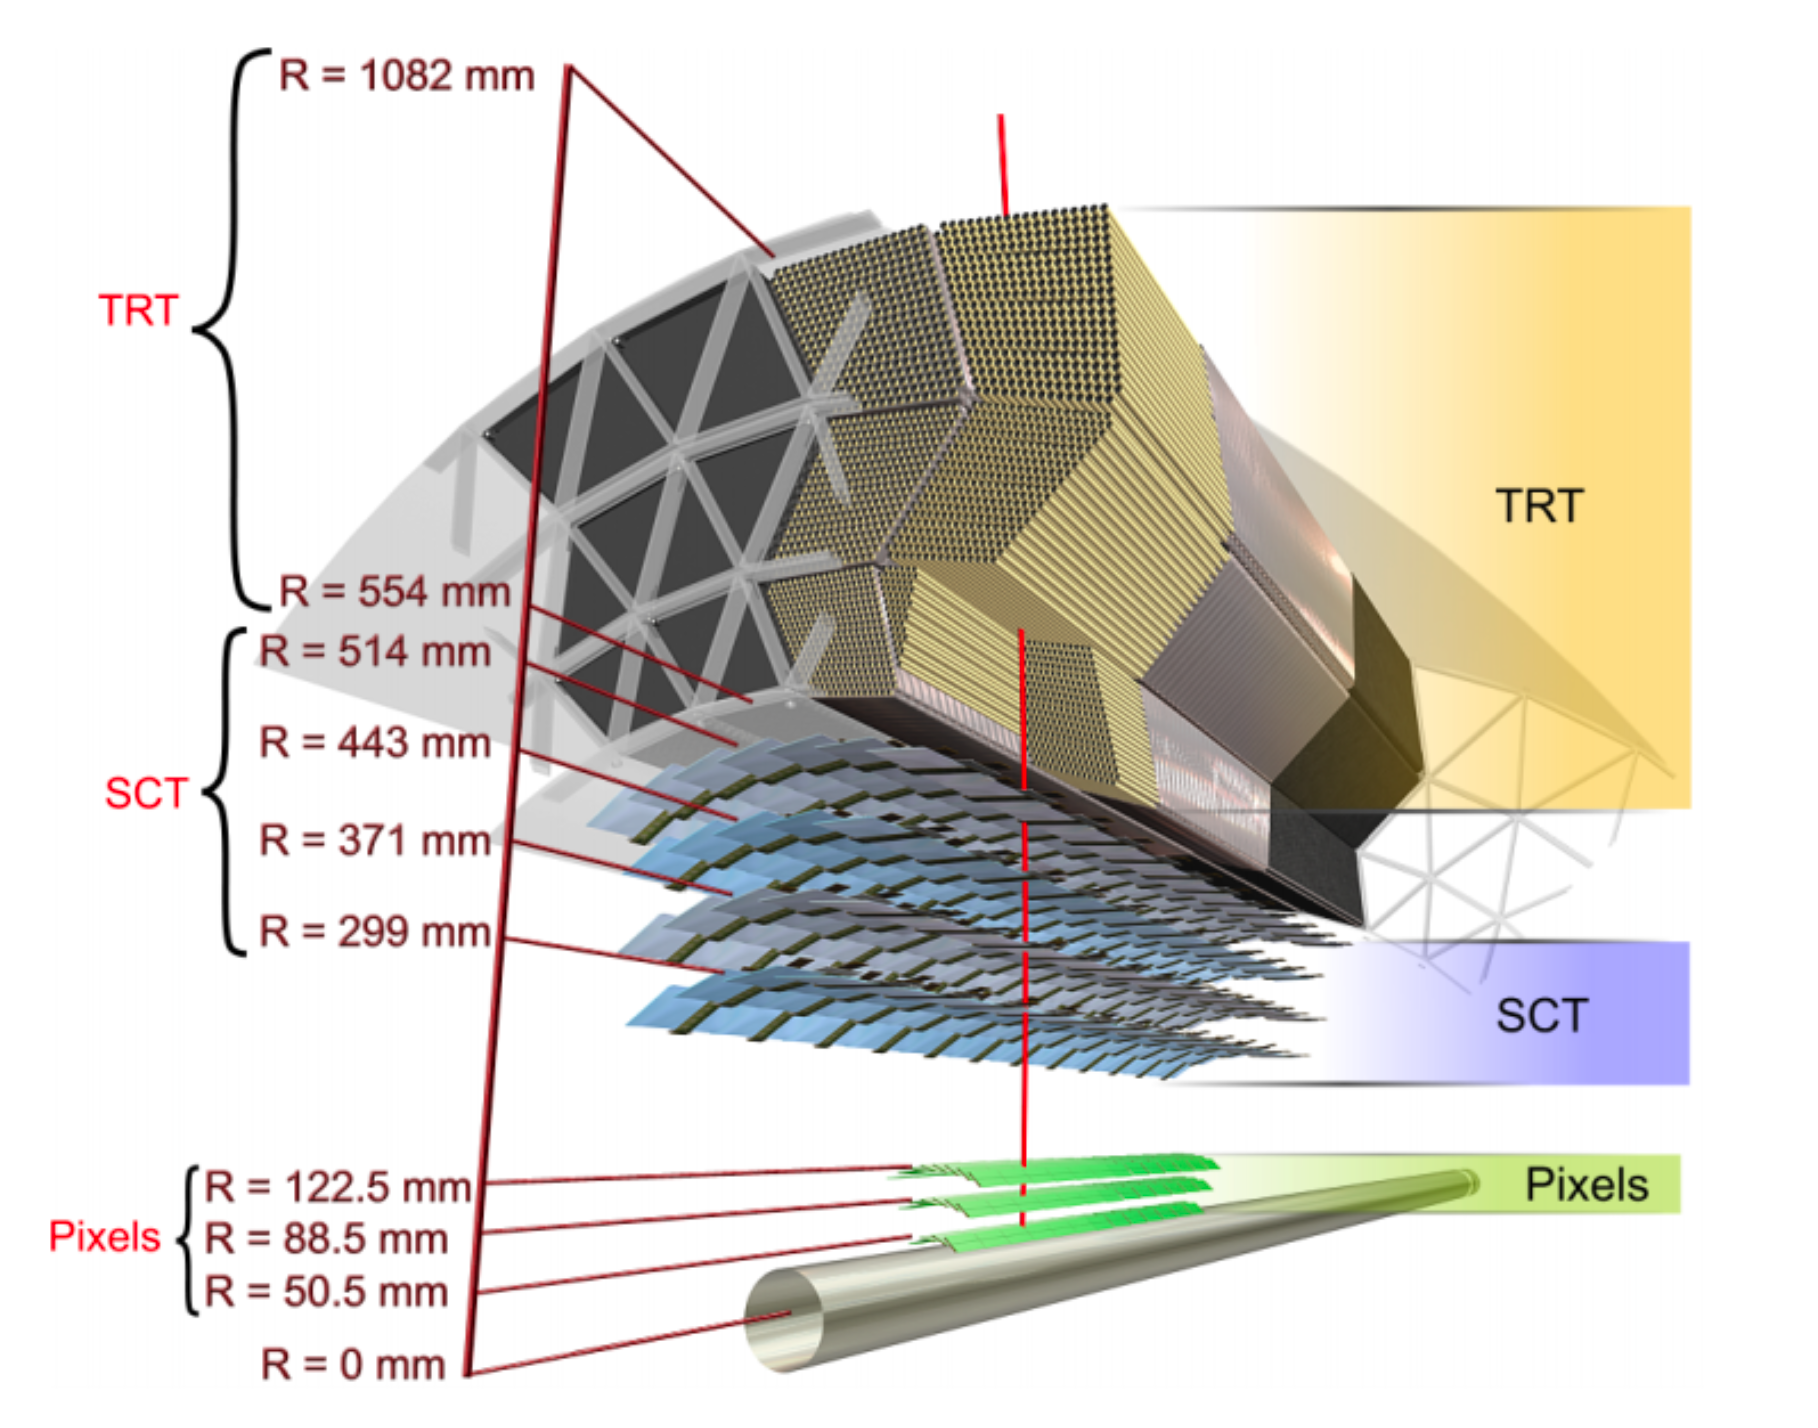
\includegraphics[width=0.5\textwidth]{data/photo/inner detector.png}
\caption{complex}
\label{fig:detector_LHC_accelerator_complex}
\end{figure}
